\documentclass{article}
\usepackage[utf8]{inputenc}
\usepackage{cite}
\usepackage{graphicx} 
\usepackage[font=small,labelfont=bf]{caption} 
\usepackage{multicol}
\usepackage{hyperref}
\usepackage{subcaption}
\usepackage{hyperref}
\usepackage{array}
\usepackage{makecell}
\usepackage[margin=0.5in]{geometry}

\hypersetup{
    colorlinks=true,
    linkcolor=blue,
    filecolor=blue,      
    urlcolor=blue,
    bookmarks=true,
    citecolor=blue
}

\usepackage[
backend=biber,
style=alphabetic,
sorting=ynt
]{biblatex}
\usepackage{lscape}

\addbibresource{bibliography.bib}


\title{Deep Learning Methods \\ Project 2}
\author{Jakub Kała \& Krzysztof Spaliński}
\date{April 2020}

\begin{document}

\maketitle

\textbf{Abstract.} The scope of the second project for Deep Learning Methods course are convolutional neural networks used in image recognition tasks. The goal is to implement and explore several network architectures and data augmentation methods. Model assessment will be carried out based on CIFAR-10 dataset.

  
\section{Documentation}
All scripts used in this project have been presented in github repository \href{https://github.com/krzysztofspalinski/deep-learning-methods-project-2}{deep-learning-methods-project-2}.

\section{CIFAR-10 Dataset}

CIFAR-10 \cite{cifar10} is a computer-vision dataset used for object recognition. In our case, it is a subset of the 80 million tiny images dataset and consists of 60,000 32x32 color images containing one of 10 object classes, with 6000 images per class. It was collected by Alex Krizhevsky, Vinod Nair, and Geoffrey Hinton.


\begin{figure}[h!]
    \centering
    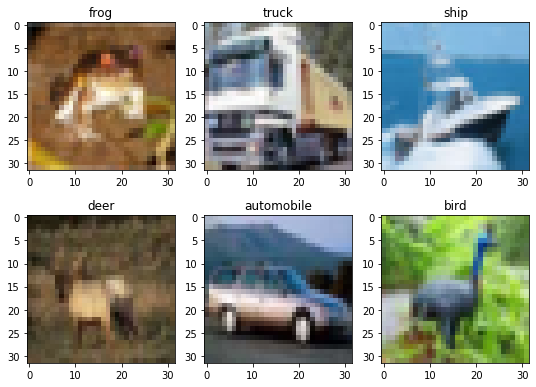
\includegraphics[width=0.8\linewidth]{data.png}
    \caption{Example images from CIFAR-10 dataset.}
\end{figure}


Dataset has been split to training and test set (50k and 10k images respectively). In order to discourage certain forms of cheating (such as hand labeling) 290,000 junk images have been added to the test set. These images are ignored in the scoring. The classes are completely mutually exclusive. 

\newpage
The label classes in the dataset are:

\begin{multicols}{2}
    \begin{itemize}
        \item airplane
        \item automobile
        \item bird
        \item cat
        \item deer 
        \item dog
        \item frog 
        \item horse
        \item ship
        \item truck
    \end{itemize}
\end{multicols}



\section{Convolutional Neural Networks}

Covolutional Neural Networks, CNNs, are neural networks employing convolution operation. They are really specialized for data with grid-like topology \cite{deeplearning}. 

Convolution is terms of neural network is operation on two tensors: input and kernel (sometimes called a filter). Researchers developed many kernels that can be used for linear image processing, for example for blurring, sharpening, detecting edges etc. In deep learning, elements of filters are trainable parameters. 


\subsection{Plain CNN architecures}
In this experiment we created three different CNN architectures, all based on VGG networks \cite{vgg} -- each network is build from blocks like this: Conv2D, BarchNorm, Conv 2D, BatchNorm, MaxPooling. Size of filters can vary, but in all architectures the number of filters increases in later layers. Last 2 layers of all networks are fully connected layers with ReLU activation function. Architectures are shown in the table blow. 

\begin{table}[h]
\centering

\begin{tabular}{|l|l|l|l|}
\hline
                               & \thead{Plain CNN 1} & \thead{Plain CNN 2} & \thead{Plain CNN 3} \\ \hline
\thead{Network \\ Architecture}
& \thead{
Conv2D 16 3x3 filters \\
BatchNorm \\ 
Conv2D 16 3x3 filters \\
BatchNorm \\ 
MaxPooling \\
Conv2D 32 3x3 filters \\
BatchNorm \\ 
Conv2D 32 3x3 filters \\
BatchNorm \\ 
MaxPooling \\
Conv2D 64 3x3 filters \\
BatchNorm \\ 
Conv2D 64 3x3 filters \\
BatchNorm \\ 
MaxPooling \\
Conv2D 128 3x3 filters \\
BatchNorm \\ 
Conv2D 128 3x3 filters \\
BatchNorm \\ 
MaxPooling \\
Dense 512 \\
Dense 512 \\
Dense 10 (softmax)
}    
&\thead{
Conv2D 16 3x3 filters \\
BatchNorm \\ 
Conv2D 16 3x3 filters \\
BatchNorm \\ 
MaxPooling \\
Conv2D 32 3x3 filters \\
BatchNorm \\ 
Conv2D 32 3x3 filters \\
BatchNorm \\ 
MaxPooling \\
Conv2D 64 3x3 filters \\
BatchNorm \\ 
Conv2D 64 3x3 filters \\
BatchNorm \\ 
MaxPooling \\
Conv2D 128 3x3 filters \\
BatchNorm \\ 
Conv2D 128 3x3 filters \\
BatchNorm \\ 
MaxPooling \\
Conv2D 256 2x2 filters \\
BatchNorm \\ 
Conv2D 512 2x2 filters \\
BatchNorm \\ 
MaxPooling \\
Dense 1024 \\
Dense 1024 \\
Dense 128 \\
Dense 10 (softmax)
}                
&\thead{
Conv2D 16 3x3 filters \\
BatchNorm \\ 
Conv2D 16 3x3 filters \\
BatchNorm \\ 
MaxPooling \\
Conv2D 32 3x3 filters \\
BatchNorm \\ 
Conv2D 32 3x3 filters \\
BatchNorm \\ 
MaxPooling \\
Conv2D 64 3x3 filters \\
BatchNorm \\ 
Conv2D 64 3x3 filters \\
BatchNorm \\ 
MaxPooling \\
Conv2D 128 3x3 filters \\
BatchNorm \\ 
Conv2D 128 3x3 filters \\
BatchNorm \\ 
MaxPooling \\
Conv2D 256 2x2 filters \\
BatchNorm \\ 
Conv2D 256 2x2 filters \\
BatchNorm \\ 
MaxPooling \\
Conv2D 512 2x2 filters \\
BatchNorm \\ 
Conv2D 512 2x2 filters \\
BatchNorm \\ 
MaxPooling \\
Dense 1024 \\
Dense 1024 \\
Dense 10 (softmax)
}                   

\\ \hline
\thead{\# \\ trainable \\ parameters} &        \thead{826k}        &          \thead{1.659kk}      &      \thead{3.843kk}    \\ \hline
\end{tabular}
\caption{Detailed information about plain CNN architectures.}
\label{architectures_info}
\end{table}


Each network was trained until there was no progress on validation set for 20 epochs. Validation set for each process of training was chosen randomly. Each architecture was trained with and without data augmentation. Training process was repeated 10 times, so there was 60 networks trained in total (3 architecturs $\times$ 2 augmentation or no augmentation $\times$ 10). Results of experiments are presented in the chart and table blow. 

\begin{center}
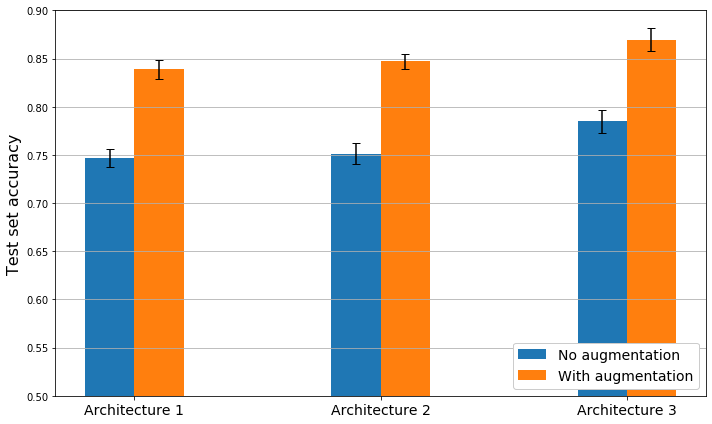
\includegraphics[scale=0.6]{results_plain_cnn.png}
\captionof{figure}{Mean accuracy and its standard deviation on the test set.}
\end{center}

\begin{table}[h]
\centering
\begin{tabular}{r|cc|cc|}
\multicolumn{1}{l|}{} & \multicolumn{2}{l|}{\textbf{No augmentation}} & \multicolumn{2}{l|}{\textbf{With augmentation}} \\
\multicolumn{1}{l|}{} & mean                  & std                   & mean                   & std                    \\ \hline
Architecture 1        & 0.747               & 0.009              & 0.838                & 0.010               \\
Architecture 2        & 0.751               & 0.011              & 0.847                & 0.008               \\
Architecture 3        & 0.784               & 0.012              & 0.869                & 0.012               \\ \hline
\end{tabular}
\caption{Detailed information about plain CNN architectures.}
\label{architectures_info}
\end{table}


As shown above, augmentation of data that CNN is trained on results in much better results on test set. We can also observe, that it does not have a visible impact on standard deviation of the results. 

The biggest network, Architecture 3, achieved the best results of accuracy on the test set. Results of Architecture 2 were slightly better than results of Architecture 1 -- Architecture 2 also had lower standard deviation (after training on augmented dataset).  

\newpage
\section{Neural network with residual blocks}

\subsection{Residual block overview}

\begin{center}
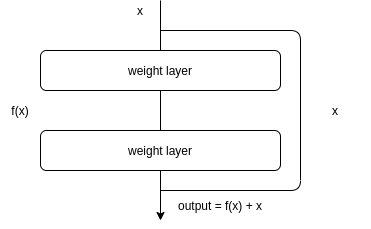
\includegraphics[scale=0.6]{resblock01.png}
\captionof{figure}{Residual block example with 2 skipped layers (source: self-made).}
\end{center}

As the neural networks start converging, a degradation problem occurs. For plain architectures, accuracy gets saturated and then degrades rapidly. This is not due to model overfitting and implementing more complex architectures does not solve the problem.
To address this issue, residual networks have been introduced in order to solve the degradation problem. Instead of fitting stacked layers, we let these layers fit a residual mapping. Formulation of this idea might be realized via implementing "shortcut connection" in a neural network.
Shortcut connections are created via an identity mapping between one or more skipped layers. Details and some mathematical background can be found in \cite{residual}.

\subsection{Experimental comparison of ResNet architectures}

In this experiment, we test 4 different architectures based on residual identity blocks. 
In these networks each residual block has 2 Conv2D layers and a skipping connection between them, but CNNs vary in their complexity. In [\ref{architectures_info}] one can find detailed information about networks: their architecture, number of trainable parameters and average time of epoch evaluation (experiments have been carried out on Tesla T4 GPU on Kaggle platform). Detailed procedure has been presented in github repository.

Experiment pipeline consists of 5 repetitions of model training, 50 epochs each. The results are further averaged and represented in [\ref{architectures_results}].





\begin{table}[ht]
\centering

\begin{tabular}{|l|l|l|l|l|}
\hline
                               & \thead{Architecture 1} & \thead{Architecture 2} & \thead{Architecture 3} & \thead{Architecture 4} \\ \hline
\thead{Network \\ Architecture}
& \thead{
Conv2D 64 filters \\
3x ResNet block (64 filters) \\
BatchNorm \& AvgPooling \\
Dense (softmax)
}    
&\thead{
Conv2D 128 filters \\
3x ResNet block (128 filters) \\
Conv2d 64 filters \\
3x ResNet block (64 filters) \\
BatchNorm \& AvgPooling \\
Dense (softmax)
}                
&\thead{
Conv2D 256 filters \\
3x ResNet block (256 filters) \\
Conv2D 128 filters \\
3x ResNet block (128 filters) \\
Conv2d 64 filters \\
3x ResNet block (64 filters) \\
BatchNorm \& AvgPooling \\
Dense (softmax)
}                   
&\thead{
Conv2d 512 filters \\
1x ResNet block (512 filters) \\
Conv2D 256 filters \\
3x ResNet block (256 filters) \\
Conv2D 128 filters \\
3x ResNet block (128 filters) \\
Conv2d 64 filters \\
3x ResNet block (64 filters) \\
BatchNorm \& AvgPooling \\
Dense (softmax)
}                  
\\ \hline
\thead{\#  trainable \\ parameters} &        \thead{107k}        &          \thead{1.07kk}      &      \thead{4.92kk}          &      \thead{10.9kk}          \\ \hline
\thead{Average \\ epoch runtime}          &        \thead{30s}        &       \thead{44s}       &    \thead{113s} &      \thead{196s}          \\ \hline
\end{tabular}
\caption{Detailed information about network architectures used in residual CNN comparison.}
\label{architectures_info}
\end{table}

\begin{table}[ht]
\centering
\begin{tabular}{|l|l|l|l|l|}
\hline
& \thead{Architecture 1} & \thead{Architecture 2} & \thead{Architecture 3} & \thead{Architecture 4} \\ \hline

\thead{Training accuracy} &$\thead{0.741 \pm 0.003}$&$\thead{0.896 \pm 0.002}$&$\thead{0.965 \pm 0.01}$&$\thead{0.976 \pm 0.002}$\\ \hline

\thead{Test accuracy} &$\thead{0.719 \pm 0.01}$&$\thead{0.829 \pm 0.017}$&$\thead{0.869 \pm 0.008}$&$\thead{0.873 \pm 0.015}$\\ \hline

\thead{Training loss} &$\thead{0.75 \pm 0.007}$&$\thead{0.301 \pm 0.005}$&$\thead{0.105 \pm 0.004}$&$\thead{0.071 \pm 0.005}$\\ \hline

\thead{Test loss} &$\thead{0.821 \pm 0.042}$&$\thead{0.532 \pm 0.065}$&$\thead{0.475 \pm 0.049}$&$\thead{0.466 \pm 0.017}$\\ \hline

\end{tabular}
\caption{Top results on CIFAR-10 dataset for each validated architecture}
\label{architectures_results}
\end{table}

In [\ref{architectures_results}] we can see that networks 1 and 2 struggle with underfitting. There is substantial difference between them and the last two architectures. Although computation complexicity for architecture 4 is much higher than for network 3, statistically, networks 3 and 4 give the same results.

There is also a visualisation of learning process presented in [\ref{plots_acc}]
and [\ref{plots_loss}] (plots with errorbars in appendix). We can see that architecture 1 is simply underfitting. Networks 3 and 4 behave in very simmilar manner. 

It is also worth noticing that we did not manage to receive significantly better results than plain CNNs.

\newpage

\begin{figure}[!h]
\begin{subfigure}{.5\textwidth}
  \centering
  % include first image
  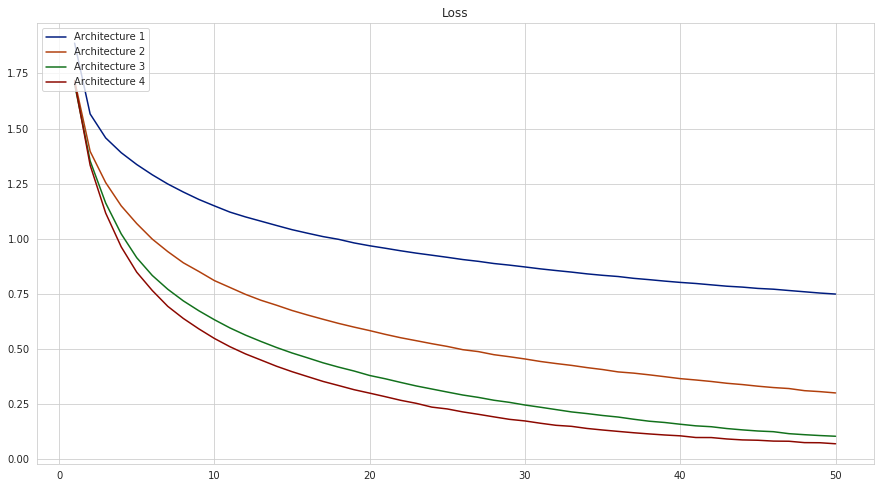
\includegraphics[width=1\linewidth]{resnet_experimentloss.png}  
  \caption{Accuracy on CIFAR-10 training set for Residual CNN architectures}
  \label{fig:sub-first}
\end{subfigure}
\begin{subfigure}{.5\textwidth}
  \centering
  % include second image
  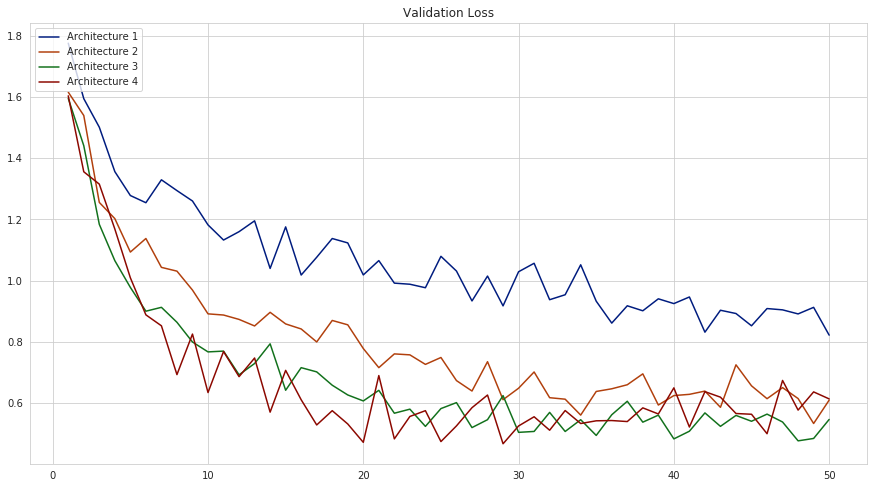
\includegraphics[width=1\linewidth]{resnet_experimentval_loss.png}  
  \caption{Accuracy on CIFAR-10 test set for Residual CNN architectures}
  \label{fig:sub-second}
\end{subfigure}
\caption{Accuracy comparison for validated CNN architectures}
\label{plots_acc}
\end{figure}








\begin{figure}[!h]
\begin{subfigure}{.5\textwidth}
  \centering
  % include first image
  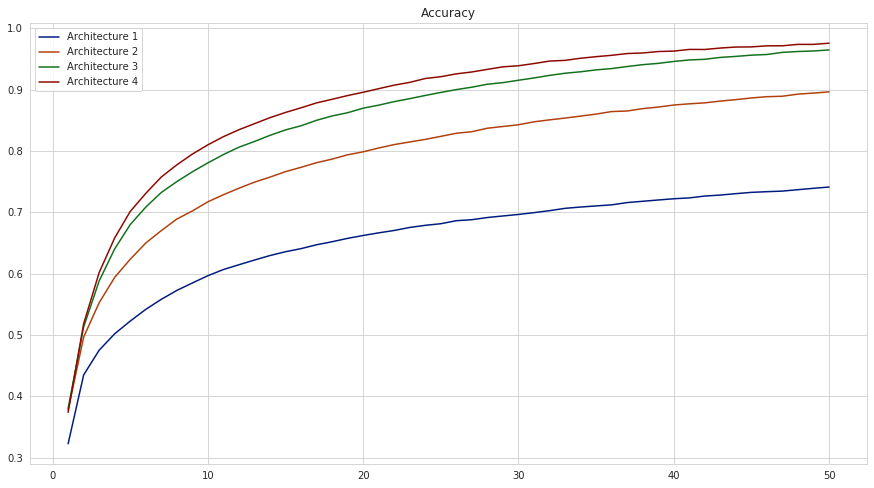
\includegraphics[width=1\linewidth]{resnet_experimentaccuracy.png}  
  \caption{Accuracy on CIFAR-10 training set for Residual CNN architectures}
  \label{fig:sub-first}
\end{subfigure}
\begin{subfigure}{.5\textwidth}
  \centering
  % include second image
  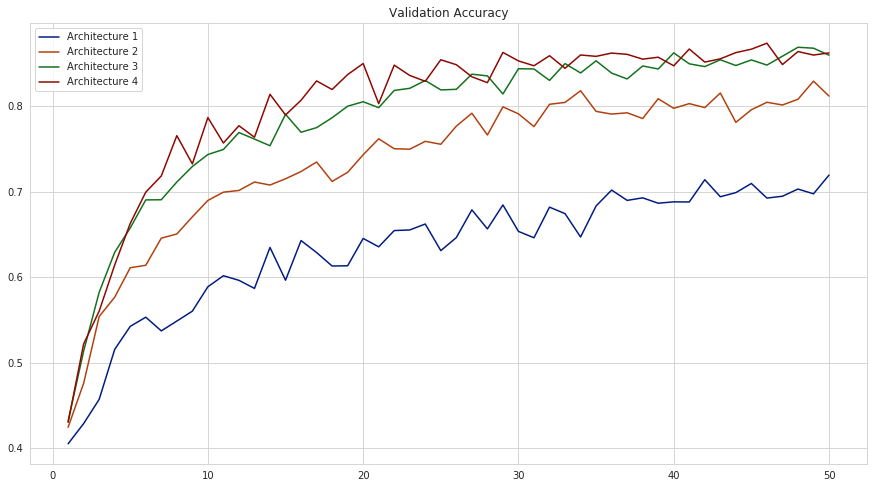
\includegraphics[width=1\linewidth]{resnet_experimentval_accuracy.png}  
  \caption{Accuracy on CIFAR-10 test set for Residual CNN architectures}
  \label{fig:sub-second}
\end{subfigure}
\caption{Accuracy comparison for validated CNN architectures}
\label{plots_loss}
\end{figure}

$\phantom{.}$

\newpage
\section{Ensemble learning for Kaggle competition}

% In order to submit predictions for CIFAR-10 dataset, we have prepared following pipeline for residual networks:
% \begin{itemize}
%     \item Architecture 4 from the experiment has been utilized
%     \item Training dataset has been randomly split into $95\%$ training and $5\%$ validation set
%     \item In order to accelerate and learning proccess, we have used Cyclical Learning Rate (details in \cite{clr})
%     \item To prevent overfitting, we have used EarlyStopping and ModelCheckpoint callbacks. We pick model that scores the best validation accuracy and the learning proccess is stopped if model does not improve for 10 epochs
%     \item 2 networks have been trained using above procedure
% \end{itemize}

In order to submit predictions for CIFAR-10 competition on Kaggle, we have used all plain CNN networks we trained (Chapter~3) to create a max voting ensemble classifier. All those networks have been trained on train test only, with randomly picked 5\% of train test as validation set and 95\% used as training data. Results are presented in the table below:

\begin{table}[h]
\begin{tabular}{l|ccc}
                                          & \begin{tabular}[c]{@{}c@{}}Only augmented networks used\\ (30 voters total)\end{tabular} & \begin{tabular}[c]{@{}c@{}}Only non-augmented networks used \\ (30 voters total)\end{tabular} & \begin{tabular}[c]{@{}c@{}}Both types of networks used \\ (60 voters total)\end{tabular} \\ \hline
\multicolumn{1}{r|}{Accuracy on test set} & 0.9107                                                                                   & 0.8467                                                                                           & 0.8952                                                                                     
\end{tabular}
\end{table}

We want to point out, that this experiment was not repeated because of its computational complexity (training of those networks on Nvidia GTX 970 took about 12 hours, making predictions took another hour). Nevertheless, results should be stable, because of the number of classifiers that took part in the voting. Screenshot from Kaggle is presented below. 

\begin{figure}[!h]
\centering
  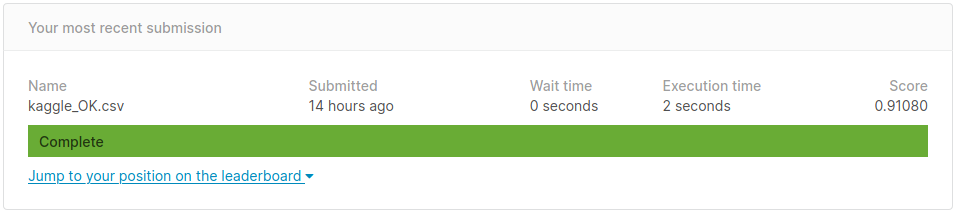
\includegraphics[width=0.6\linewidth]{kaggle.png}  
\caption{Screenshot with our accuracy score from Kaggle.}
\label{kaggle}
\end{figure}


The result can be reproduced using \href{https://github.com/krzysztofspalinski/deep-learning-methods-project-2/blob/master/notebooks/eksperyment-plain-cnn.ipynb}{this notebook} to train networks. Trained models can be found \href{https://drive.google.com/drive/folders/1nLcQi99gMlS13X3SBfsNG3rxye-Ux5ZH?usp=sharing}{here}. Notebook that makes prediction on Kaggle test set can be found \href{https://github.com/krzysztofspalinski/deep-learning-methods-project-2/blob/master/notebooks/kaggle_submission.ipynb}{here}. The final solution CSV file is \href{https://github.com/krzysztofspalinski/deep-learning-methods-project-2/blob/master/results/kaggle_OK.csv}{here}.


\vspace{20em}
\printbibliography


\section{Appendix}
\subsection{Experiment results with error bars}

Learning histories for each architecture from ResNet experiment with error bars attached can be found in [\ref{err1}, \ref{err2}, \ref{err3}, \ref{err4}]

\begin{figure}[!h]
  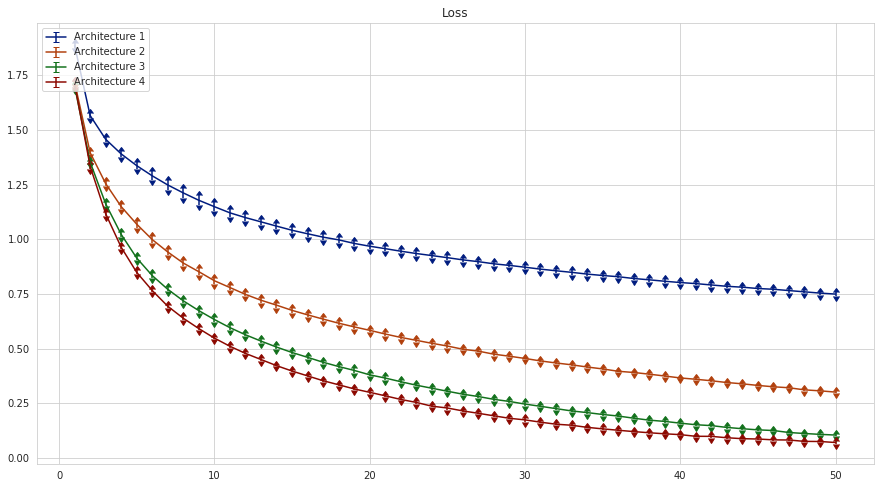
\includegraphics[width=1\linewidth]{resnet_experimentloss_errorbars.png}  
\caption{Residual networks experiment - Loss with errors}
\label{err1}
\end{figure}

\begin{figure}[!h]
  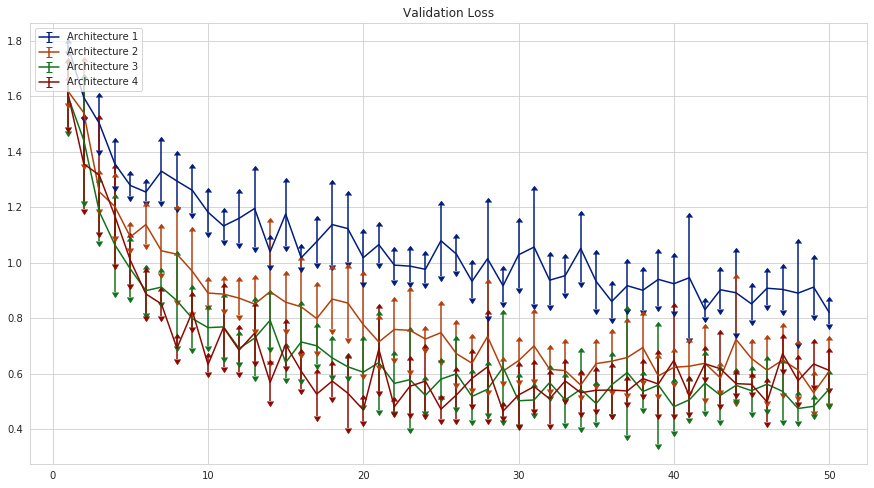
\includegraphics[width=1\linewidth]{resnet_experimentval_loss_errorbars.png}  
\caption{Residual networks experiment - Validation loss with errors}
\label{err2}
\end{figure}

\begin{figure}[!h]
  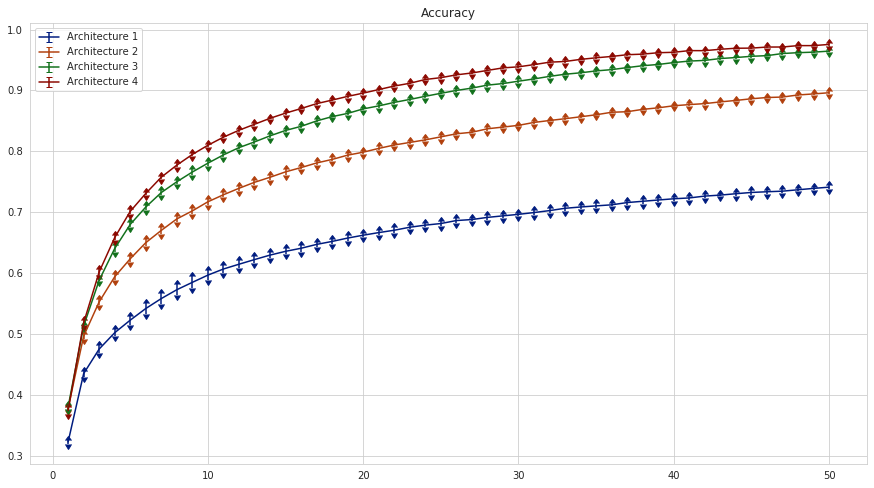
\includegraphics[width=1\linewidth]{resnet_experimentaccuracy_errorbars.png}  
\caption{Residual networks experiment - Accuracy with errors}
\label{err3}
\end{figure}

\begin{figure}[!h]
  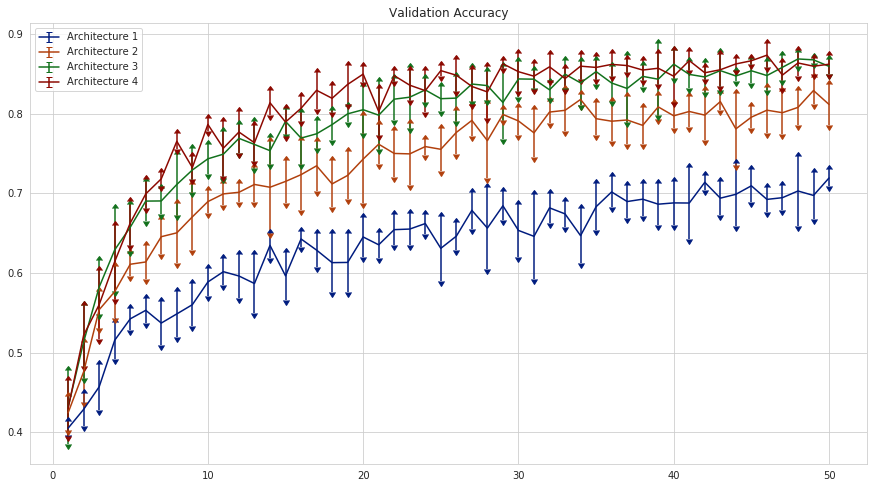
\includegraphics[width=1\linewidth]{resnet_experimentval_accuracy_errorbars.png}
\caption{Residual networks experiment - Validation accuracy with errors}
\label{err4}
\end{figure}


\end{document}
